\documentclass{beamer}
\usetheme{Madrid}
%\usecolortheme{seahorse}
\usepackage[utf8]{inputenc}
\usepackage[portuguese]{babel}
\usepackage{fouriernc,DejaVuSans,graphicx,xcolor}
\usepackage[T1]{fontenc}
\setlength{\parindent}{0pt}
\setlength{\parskip}{12pt}
\definecolor{brown}{rgb}{0.75,0.55,0.1}
\definecolor{violet}{rgb}{0.7,0.1,0.8}
\definecolor{blue}{rgb}{0,0,0.9}

\title{Introdução ao LaTeX -- Primeira parte}
\author{Jaime Villate}
\institute[FEUP]{Faculdade de Engenharia da Universidade do Porto}
\date[29/11/2021]{29 de novembro de 2021}

\begin{document}
\frame{\titlepage}
\begin{frame}
\frametitle{Conteúdo}
\tableofcontents
\end{frame}
\section{Introdução}
\begin{frame}
  \frametitle{Introdução}
  Sistema para criar documentos.\\
  \includegraphics[width=0.5\textwidth]{samples/tese.png}\hfill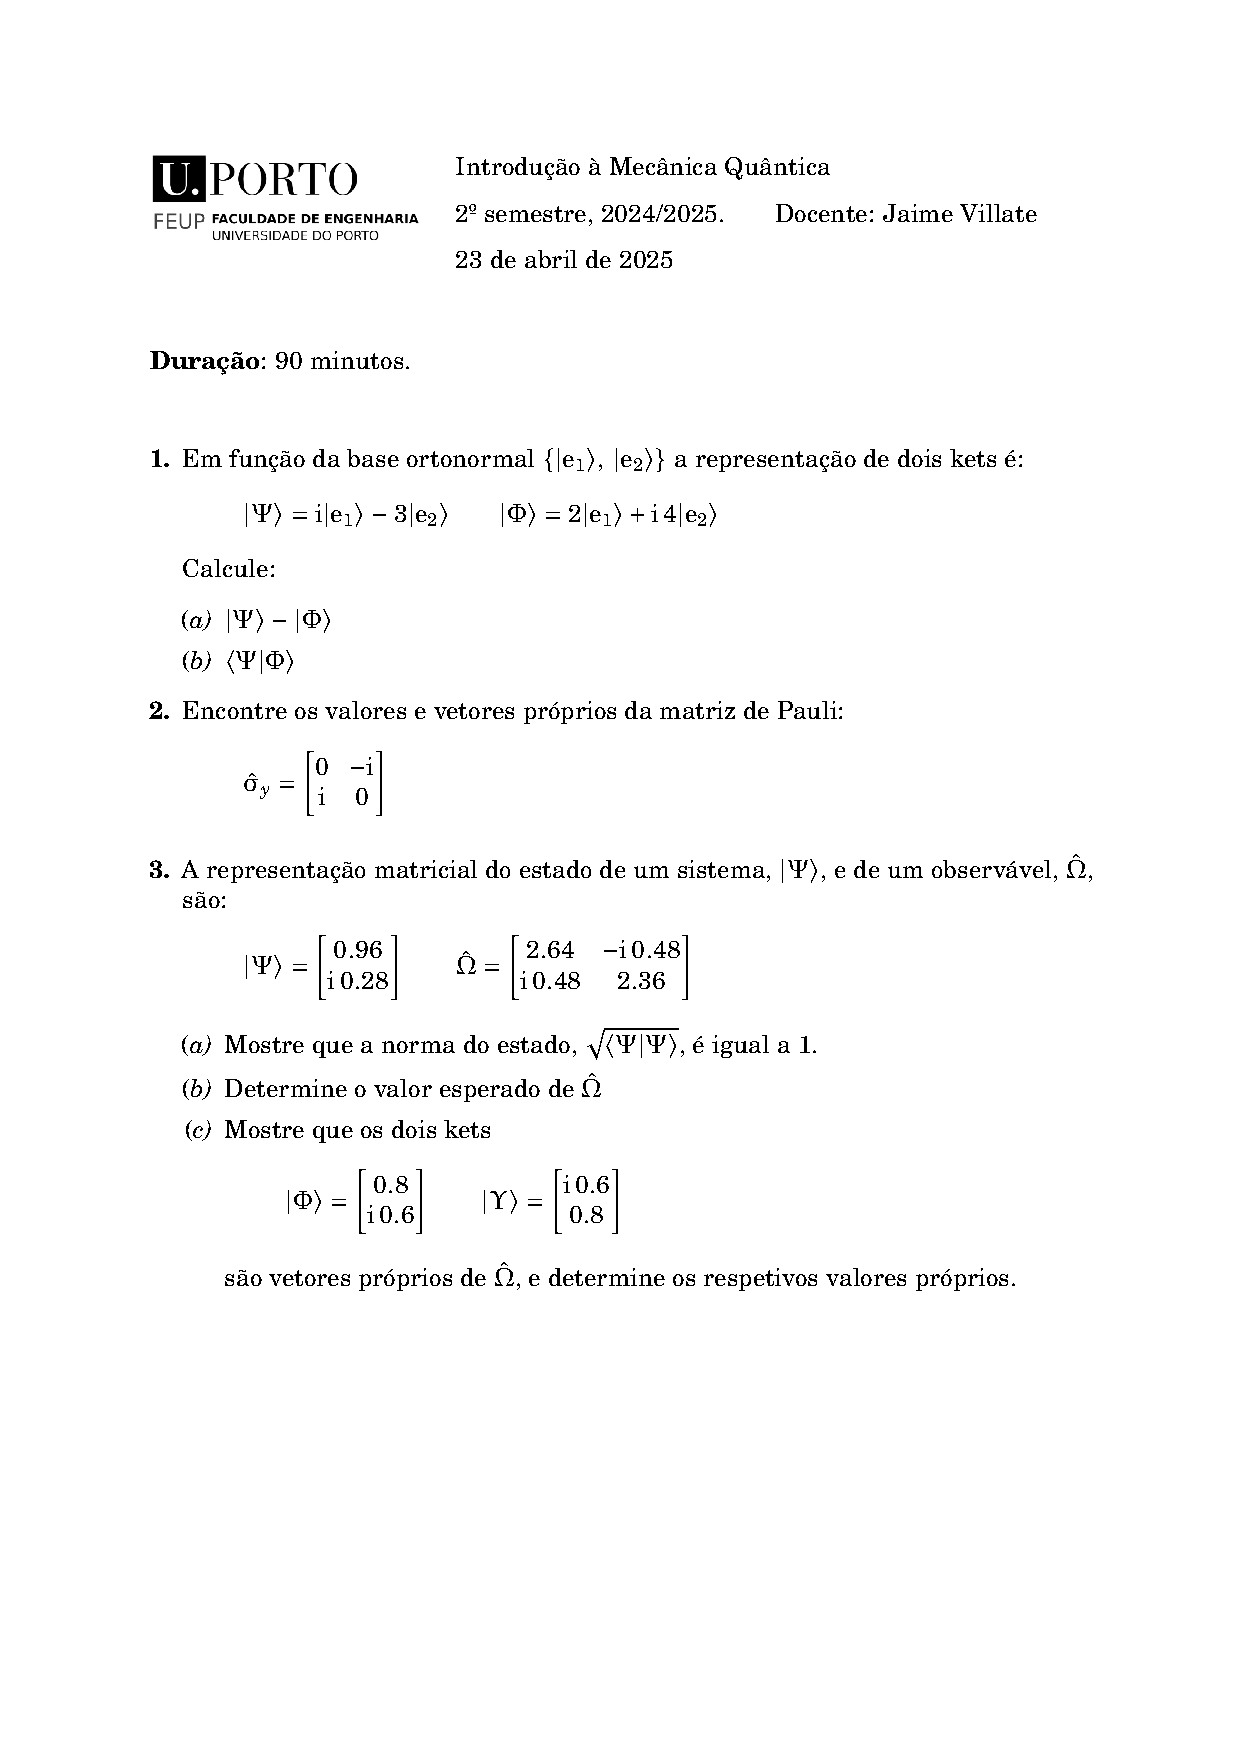
\includegraphics[width=0.44\textwidth]{samples/exame.png}
\end{frame}
\section{Vantagens e desvantagens}
\begin{frame}
  \frametitle{Vantagens}
  \begin{itemize}
  \item<1-> Ênfase no conteúdo, e não na formatação.
  \item<2-> Reaproveitamento dos documentos.
  \item<3-> Formatação consistente e mais uniforme.
  \item<4-> Facilidade de alterações globais ao documento.
  \item<5-> Biblioteca muito extensa de pacotes e documentos
    (\url{https://ctan.org/}).
  \item<6-> Possibilidade de ser usado em muitos sistemas diferentes.
  \item<7-> Facilidade de automatizar tarefas.
  \item<8-> Fácil conversão para outras linguagens, como HTML.
  \end{itemize}
\end{frame}
\begin{frame}
  \frametitle{Desvantagens}
  \begin{itemize}
  \item<1-> Necessidade de processar ficheiros fonte.
  \item<2-> Documentos não criados por erros no ficheiro fonte.
  \item<3-> Sistema complexo de criação de estilos de documento.
  \item<4-> Escrever um documento é escrever um programa.
  \end{itemize}
\end{frame}
\section{Estilos de documento}
\begin{frame}
  \frametitle{Ficheiros fonte}
  Normalmente com extensão \texttt{.tex}. Ficheiros de texto simples.\pause
    
  Parágrafos separados por uma ou mais linhas em branco.\pause

  Espaços ou fim de linha adicionais não alteram um parágrafo.\pause

  \vspace*{12pt}
  \begin{block}{Caracteres especiais}
    \qquad$\backslash$\quad \%\quad \&\quad \#\quad \$\quad \_\quad
    $\sim$\quad $\wedge$\quad \{\quad \}\quad [\quad ]
  \end{block}
\end{frame}
\begin{frame}
  \frametitle{Processamento}
  O ficheiro fonte deve ser processado pelo programa
  \textcolor{blue}{latex} ou equivalente (\textcolor{blue}{pdflatex},
  \ldots) para produzir o documento.\pause

  Alguns sistemas já incorporam um editor de texto para o ficheiro fonte,
  e botões para executar os programas necessários.\pause

  Os programas necessários deverão estar instalados no
  computador.\pause

  São criados alguns ficheiros auxiliares (\texttt{.log},
  \texttt{.aux}, \ldots).\pause
  
  Pode também usar-se um sistema \emph{on-line} como, por exemplo,
  \url{https://www.overleaf.com}
\end{frame}
\section{Pacotes}
\begin{frame}
  \frametitle{Exemplo}
  Disponível em: \url{https://www.overleaf.com/read/hctqddrtmbzg}
  
  \begin{center}
    \includegraphics{samples/doc1.png}
  \end{center}

  Estrutura dos comandos: \textcolor{violet}{$\backslash$comando} [\textcolor{brown}{opções}] \{\textcolor{blue}{nome}\}
  
  \textcolor{violet}{documentclass} identifica o \textbf{estilo
    do documento} e \textcolor{violet}{usepackage} permite usar
  \textbf{pacotes} adicionais.
\end{frame}
\section{Formatação}
\begin{frame}
  \frametitle{Tipos de texto}
  \begin{itemize}
  \item<1-> Itálica: \textcolor{violet}{$\backslash$emph}\{texto\}
  \item<2-> Negrita: \textcolor{violet}{$\backslash$textbf}\{texto\}
  \item<3-> Sublinhado: \textcolor{violet}{$\backslash$underline}\{texto\}
  \item<4-> Tamanho constante: \textcolor{violet}{$\backslash$texttt}\{texto\}
  \end{itemize}
\end{frame}
\section{Figuras}
\begin{frame}
  \frametitle{Figuras}
  Usa-se o pacote \textcolor{blue}{graphicx} no preâmbulo e o comando
  \textcolor{violet}{includegraphics} para inserir uma imagem.\pause

  \textcolor{violet}{$\backslash$includegraphics}\{roda.png\} insere a imagem
  \includegraphics[scale=0.05]{doc/roda.png} na linha de texto.\pause

  Dentro de
  \textcolor{violet}{$\backslash$begin}\{\textcolor{blue}{center}\}
  e \textcolor{violet}{$\backslash$end}\{\textcolor{blue}{center}\}, a
  imagem aparece centrada, fora do texto:\pause
  \begin{center}
    \includegraphics[width=0.4\textwidth]{doc/roda.png}
  \end{center}
\end{frame}
\begin{frame}
  \frametitle{Comando includegraphics}
  Importa figuras JPG, PNG, PDF ou Postscript.\pause

  Algumas opções:
  \begin{itemize}
  \item<2-> $[$\textcolor{brown}{height=1cm}$]$ Altura da imagem.
  \item<3-> $[$\textcolor{brown}{width=1cm}$]$ Largura da imagem.
  \item<4-> $[$\textcolor{brown}{scale=0.2}$]$ Fator de redução do tamanho.
  \item<5-> $[$\textcolor{brown}{angle=90}$]$ Rotação em graus.
  \end{itemize}
\end{frame}
\section{Listas}
\begin{frame}
  \frametitle{Listas de itens}
  Exemplo:

  \begin{itemize}
  \item item 1.
  \item item 2.
  \item item 3.
  \end{itemize}

  \pause

  Foi obtida com o texto: \qquad
  \raisebox{-20pt}{\includegraphics[scale=1.2]{samples/itemize.png}}\pause

  O ``bullet'' usado é definido pelo estilo do documento.
\end{frame}
\begin{frame}
  \frametitle{Listas enumeradas}
  Exemplo:

  \begin{enumerate}
  \item item 1.
  \item item 2.
  \item item 3.
  \end{enumerate}

  \pause
  Foi obtida com o texto: \qquad
  \raisebox{-20pt}{\includegraphics[scale=1.2]{samples/enumerate.png}}\pause

  O tipo de números usados é definido pelo estilo do documento.
\end{frame}
\begin{frame}
  \frametitle{Listas descriptivas}
  Exemplo:

  \begin{description}
  \item[primeiro:] Descrição 1.
  \item[segundo:] Descrição 2.
  \item[terceiro:] Descrição 3.
  \end{description}

  \pause
  Foi obtida com o texto: \qquad
  \raisebox{-20pt}{\includegraphics[scale=1.2]{samples/description.png}}\pause

  A formatação da lista é definida pelo estilo do documento.
\end{frame}
\end{document}
